\documentclass[12pt]{article}
\usepackage[a4paper, total={6in, 10in},top=10mm, bottom=5mm]{geometry}
\usepackage{hyperref}
\usepackage{pgfgantt}


\usepackage{graphicx}
\graphicspath{{../../images/}}

\usepackage[counterclockwise]{rotating} %sidewaysfigure

\title{ Are Robots the Future of Elder Care?  } 
\author{Miguel P Xochicale \\
https://github.com/mxochicale/3mt}
\date{\today}

\begin{document}
\maketitle

If you are lucky enough, you will live to an average of 80 years.
But, have you ever wondered what it would be like turning 70, 80 or maybe 90 years old?
Now, imagine as we age, we will be gradually losing all of our
charming human senses such as sight, hearing, taste, smell, and touch.
In short, both our cognitive and motor skills will diminish as we age.

Now think about the people who will be with you until the last day of your life.
Will they be with you at all 
and most importantly will they take care of you?

And how about the global view of people who are aging.
According to the 2017 revision of the world population prospects \cite{un2017}, 
people age 60 years or over
are expected to be more than double by 2050 and to be more than triple by 2100 \cite{unb2017}.

Well, you don`t have to worry too much in the coming years, 
because this is where caregiver robots and MY RESEARCH come in.

In my PhD, 
I have created a novel analysis and interpretation of nonlinear time series
for movement variability.
Particularly,
I have studied, understood and implemented algorithms of nonlinear dynamics
in order to measure human movement variability.
I have also conducted experiments in the context of human robot-interaction 
where people follow upper arm movements performed by a robot 
in order to test the algorithms that measure movement variability \cite{xochicale2018}.

Applications of my research are many but let me give you two examples
* In the last five years, 
robots like Palro, a small humanoid robot, can play games and dance with the elder
and therefore keep their minds active.
* Another one is Pepper, a personal humanoid robot,  has the power 
to read and respond to human emotions \cite{hay2015}.

Both of the previous examples offer no feedback to people's movement when 
interacting with the humanoid robots.

So, in the near future, caregiver robots will gradually meet our physical and emotional needs as we age, 
by encouraging social activities, healthy eating and exercise \cite{aronson2014}.
That is the future that I am working on.
A future where humanoid robots can automatically enhance and monitor physical activities of the elderly.

Perhaps my parents, back in Mexico, are not going to directly benefit 
from these technological advances 
but I do believe that 
future generations of people world-wide
will be assisted by caregiver robots,
therefore making the elderly more independent, happier and healthier!


\newpage



\section*{Key Dates} 

\begin{ganttchart}[
	hgrid,
	vgrid,
	x unit=1mm,
	time slot format=isodate-yearmonth
	]{2018-03-01}{2018-05-31}
%\gantttitlecalendar{year,month=shortname,week} \\
\gantttitlecalendar{year,month=shortname} \\
%\ganttbar{rehearsals}{2018-03-02}{2018-04-30} \\
\ganttmilestone{training at BrH (26) }{2018-03-26} \\
\ganttmilestone{training at UoB (19) }{2018-04-19} \\
\ganttmilestone{drop-in at GK-N224 (26) }{2018-04-19} \\

\ganttmilestone{submit-slide (01-15h00m) }{2018-05-02} \\
\ganttmilestone{heat-practice (02-12h00m) }{2018-05-02} \\
\ganttmilestone{heat (03) }{2018-05-03} \\
\ganttmilestone{bham-final (16) }{2018-05-16} 
\end{ganttchart}



\section*{Acknowledgements}

I would like to acknowledge to the following people
who helped me to improve the script.
To Georgina Hardy and Eren Bilgen for the feedback in the training and drop in for 
the 3 minute thesis competition. To my English teachers at the brasshouse and to 
the one to one tutorials at University of Birmingham. 
Last but not least to Isabella Fritz who gave acute feedback 
in order to polish and refining the script.

%\begin{sidewaysfigure}
%\centering
%\includegraphics{figure02}
%\caption{3 minutes thesis figure}
%\end{sidewaysfigure}




%\newpage

\begin{thebibliography}{10}

\bibitem{hay2015}
Mark Hay,
{\it Why robots are the future of elder care?},
{\url{https://www.good.is/articles/robots-elder-care-pepper-exoskeletons-japan}} (24 June 2014)


\bibitem{un2017}
United Nations,
{\it The 2017 Revision of the World Population Prospects},
{\url{https://esa.un.org/unpd/wpp/Publications/Files/WPP2017_KeyFindings.pdf}}


\bibitem{unb2017}
United Nation Blog,
{\it Ageing},
{\url{http://www.un.org/en/sections/issues-depth/ageing}} (24 June 2014)


\bibitem{matuszek2017}
Cynthia Matuszek,
{\it Robot caregivers for the elderly could be 10 years away},
{\url{http://uk.businessinsider.com/robot-caregivers-for-the-elderly-10-years-away-2017-8}} (28 August 2017)


\bibitem{aronson2014}
Louise Aronson,
{\it The future of robot caregivers},
{\url{https://www.nytimes.com/2014/07/20/opinion/sunday/the-future-of-robot-caregivers.html}} (19 July 2014)



\bibitem{xochicale2018}
Miguel P Xochicale,
{\it Publications},
{\url{https://mxochicale.github.io/publications}}


\end{thebibliography}



\end{document}
